\chapter{REST e Docker}

\section{REST}

\subsection{Introduzione}

\dfn{REST}{
	REST è uno stile architetturale per creare APIs in rete: specifica la forma e la semantica della comunicazione tra un provider (server) e un consumer (client).
}

\nt{REST sta per REpresentional State Transfer.}

\clm{}{}{
	\begin{itemize}
		\item Il provider fornisce \fancyglitter{risorse concettuali}.
		\item Il consumer può manipolare una risorsa scambiando sue rappresentazioni.
		\item Le interazioni avvengono mediante richieste \fancyglitter{stateless} con un interfaccia uniforme (HTTP, URI, etc.).
		\item Solitamente si implementa con HTTP (mappa naturalmente con i principi REST).
		\item Sia il provider che il consumer devono essere \fancyglitter{compliant} con la specifica API concordata.
	\end{itemize}
}

\cor{REST Resources}{
	Gli Endpoint URIs (pathname) dovrebbero esprimere risorse (nomi), non azioni. Mappano sui DDD:
	\begin{itemize}
		\item Part di path rappresentano entità (tipi + id).
		\item Path annidate rappresentano oggetti aggregati o contenuti.
	\end{itemize}
}

\begin{figure}[h]
	\centering
	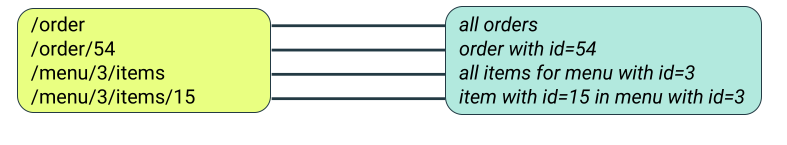
\includegraphics[scale=0.6]{02/rest res.png}
	\caption{Esempio di mappatura REST resources su DDD.}
\end{figure}

\subsection{Verbi e Status Responses}

\cor{REST Verb}{
	I verbi esprimono le azioni effettuate su una risorsa. I verbi di REST mappano su metodi HTTP.
}

\paragraph{I verbi:}

\begin{itemize}
	\item GET ottiene una rappresentazione di una risorsa specifica (legge dei dati):
	      \begin{itemize}
		      \item Non ha side effects ed è idempotente.
		      \item Non ha un body.
		      \item \fancyglitter{Query String:} usata per aggiungere filtri sulla richiesta.
	      \end{itemize}

	      \begin{figure}[h]
		      \centering
		      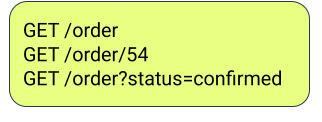
\includegraphics[scale=0.65]{02/GET.png}
		      \caption{REST GET.}
	      \end{figure}

	\item POST viene usata per creare una nuova risorsa:
	      \begin{itemize}
		      \item Ha side effects e non è idempotente.
		      \item Il body contiene la rappresentazione della nuova risorsa.
		      \item \fancyglitter{Query String:} usata per esprimere modificatori per la richiesta.

	      \end{itemize}

	      \begin{figure}[h]
		      \centering
		      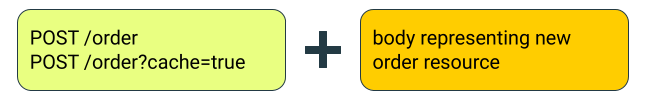
\includegraphics[scale=0.65]{02/POST.png}
		      \caption{REST POST.}
	      \end{figure}

	\item PUT rimpiazza una risorsa esistente con una nuova rappresentazione:
	      \begin{itemize}
		      \item Ha side effects, ma è idempotente.
		      \item Il body contiene una rappresentazione aggiornata della risorsa.
		      \item \fancyglitter{Query String:} usata per aggiungere filtri sulla richiesta (come in POST).

	      \end{itemize}

	      \begin{figure}[h]
		      \centering
		      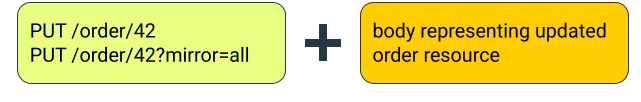
\includegraphics[scale=0.65]{02/PUT.png}
		      \caption{REST PUT.}
	      \end{figure}

	\item DELETE cancella una risorsa esistente:
	      \begin{itemize}
		      \item Ha side effects, ma è idempotente.
		      \item Non ha un body (come in GET).
		      \item \fancyglitter{Query String:} usata per aggiungere filtri sulla richiesta (come in POST).

	      \end{itemize}
	       \begin{figure}[h]
		      \centering
		      
\includegraphics[scale=0.65]{02/DELETE.png}
		\caption{REST DELETE.}
	      \end{figure}


	\item PATCH aggiorna solo una parte della risorsa:
	      \begin{itemize}
		      \item Ha side effects, può essere idempotente o meno (dipende dal tipo di aggiornamento).
		      \item Il body contiene o una rappresentazione parziale delle risorse o i cambiamenti applicati.
		      \item \fancyglitter{Query String:} usata per aggiungere filtri sulla richiesta (come in POST).

	      \end{itemize}
	       \begin{figure}[h]
		      \centering
		      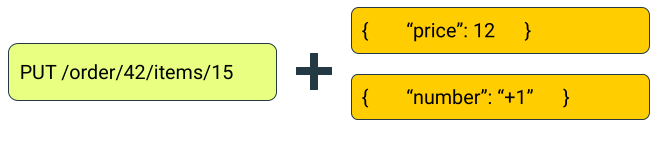
\includegraphics[scale=0.65]{02/PATCH.png}
		\caption{REST DELETE.}
	\end{figure}
\end{itemize}

\dfn{REST Status Responses}{

	REST associa specifici significati agli status code che devono essere rispettati per la compliance.
}

\paragraph{Risposte:}

\begin{itemize}
	\item 2XX - Successo:
	      \begin{itemize}
		      \item 200 - OK: successo generico.
		      \item 201 - Created: una POST che ha creato con successo una nuova risorsa.
		      \item 204 - No Content: operazione che ha avuto successo ma non ha restituito un body (DELETE o PUT).
	      \end{itemize}
	\item 3XX - Redirezione:
	      \begin{itemize}
		      \item 303 - See Other: dopo che una POST redirige a una GET della risorsa creata.
	      \end{itemize}
	\item 4XX - Errore Client:
	      \begin{itemize}
		      \item 400 - Bad Request: la richiesta è malformata.
		      \item 401 - Unauthorized: credenziali mancanti o invalide.
		      \item 403 - Forbidden: l'utente è autenticato, ma non è autorizzato ad accedere a tali risorse.
		      \item 404 - Not Found: la risorsa desiderata non esiste.
		      \item 409 - Conflict: lo stato attuale del sistema è in conflitto con l'operazione (per business rulles, etc.)
		      \item 422 - Unprocessable Entity: la richiesta viola delle regole semantiche.
		      \item 429 - Too Many Requests - superà il limite di richieste possibili\footnote{Indovinate chi è stata bannata dall'AUR per aver spammato richieste LOL.}.
	      \end{itemize}
	\item 5XX - Errore Server:
	      \begin{itemize}
		      \item 500 - Internal Server Error: eccezione generica.
		      \item 502 - Bad Gateway: il servizio fallisce per via di un fallimento upstream (proxies).
		      \item 503 - Service Unavailable: servizio temporaneamente down.
		      \item 504 - Gateway Timeout: timeout upstream (proxies).
	      \end{itemize}
\end{itemize}

\paragraph{REST vs. RPC:}

\begin{itemize}
	\item REST: gli endpoint identificano risorse, i verbi dicono cosa fare con essere e il body rappresenta la rappresentazione delle risorse.
	\item RPC: gli endpoint esprimono le operazioni da fae e il body rappresenta i parametri ( nella richiesta) o il valore restituito (nella risposta).
\end{itemize}

\paragraph{Pragmatic REST:}

\begin{itemize}
	\item Anche usando i verbi a volte è necessario che gli endpoint esprimano operazioni:
	      \begin{itemize}
		      \item Quando la semantica operazionale è a grana  troppo fine per essere limitata ai verbi. 
		      \item Quando le operazioni non corrispondono a risorse esistenti nel server.
	      \end{itemize}
      \item Si può provare a rimanere REST:
	      \begin{itemize}
		      \item Piazzando il verbo dopo l'identificazione della risorsa. 
		      \item Rispettando la caratterizzazione del verbo.
	      \end{itemize}
\end{itemize}

\qs{}{Dove usiamo REST in un'architettura a microservizi?}

\begin{figure}[h]
	\centering
	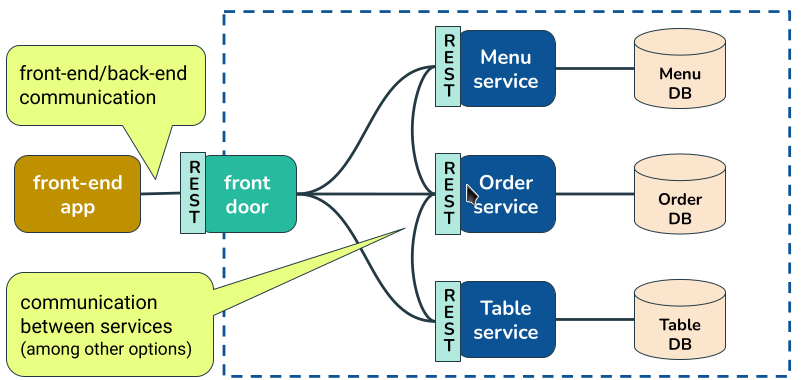
\includegraphics[scale=0.25]{02/msa.png}
	\caption{Utilizzo di REST in MSOAs.}
\end{figure}

\dfn{External Exposed API}{
API che sono esposte al mondo, Solitamente con un  gateway che blocca l'accesso. 
}

\dfn{Internal Service API}{
API interne all'applicazione con un ingresso.
}

\nt{L'ingresso pubblica quello che esiste, il gateway si occupa di cosa esporre.}

\begin{figure}[h]
	\centering
	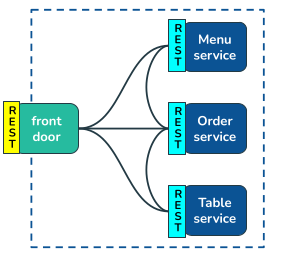
\includegraphics[scale=0.6]{02/API.png}
	\caption{Relazione tra API interne ed esterne.}
\end{figure}

\section{Docker}








